\documentclass{article}

\usepackage[margin=0.5in]{geometry}
\usepackage{multicol}
\usepackage{amsthm}
\usepackage{amsmath}
\usepackage{tikz}
\usetikzlibrary{quotes,angles}

\theoremstyle{definition}
\newtheorem*{solution}{Solution}
\title{Plane Geometry Set A}
\date{}
\author{}

\begin{document}
\maketitle

\begin{multicols}{2}
    \begin{enumerate}
        \item In quadrilateral $ABCD$, the measure of angle $A$ is half the sum of the measures of the other angles.
            What is the measure of angle $A$?
            Express your answer to the nearest integer.
            \begin{solution}
                The sum of the angle measures in a quadrilateral is $360^{\circ}$.
                Let's say the sum of the measures of angles $B$, $C$, and $D$ is $x$.
                The measure of angle $A$ is half of that, or $\frac{1}{2}x$, so $360 = \frac{1}{2}x + x = \frac{3}{2}x$.
                This means $x = 360 \div \frac{3}{2} = 360 \cdot \frac{2}{3} = 240$ and $A = \frac{1}{2} \cdot 240 = 120^{\circ}$.
            \end{solution}
        \item The two circles in the figure are tangent at $G$.
            Prove that $\angle E = \angle F$.
            \begin{center}
                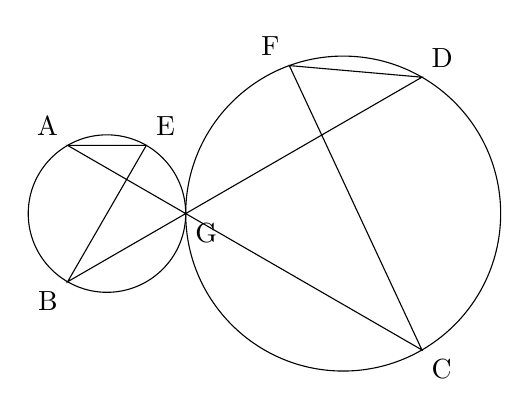
\begin{tikzpicture}
                    \draw (0,0) circle (1cm);
                    \coordinate[label=above left:A] (A) at (120:1);
                    \coordinate[label=below left:B] (B) at (240:1);
                    \coordinate[label=above right:E] (E) at (60:1);
                    \coordinate[label=below right:G] (G) at (1,0);
                    \begin{scope}[shift={(3,0)}]
                        \draw (0,0) circle (2cm);
                        \coordinate[label=above left:F] (F) at (110:2);
                        \coordinate[label=above right:D] (D) at (60:2);
                        \coordinate[label=below right:C] (C) at (300:2);
                    \end{scope}
                    \draw (A) -- (E) -- (B) -- (G) -- (D) -- (F) -- (C) -- (G) -- cycle;
                \end{tikzpicture}
            \end{center}
            \begin{solution}
                Since $\angle AGB$ and $\angle DGC$ are vertical angles, they are equal.
                Since $\angle F$ and $\angle DGC$ are inscribed angles which subtend the same arc, they are equal.
                Finally, $\angle E = \angle AGB$ because they are inscribed angles subtending the same arc.
                Thus, $\angle E = \angle AGB = \angle DGC = \angle F$.
            \end{solution}
        \item Triangle $ABC$ is inscribed in a semicircle as shown.
            If $m\angle ABC = 24^{\circ}$, what is the degree measure of $\angle BCA$?
            \begin{center}
                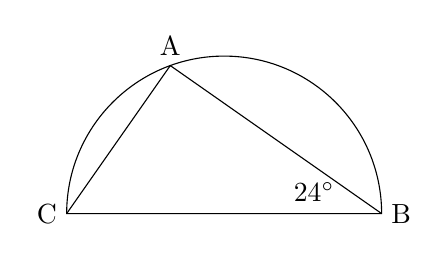
\begin{tikzpicture}
                    \draw (2,0) arc (0:180:2cm) -- cycle;
                    \coordinate[label=above:A] (A) at (110:2);
                    \coordinate[label=right:B] (B) at (2,0);
                    \coordinate[label=left:C] (C) at (-2,0);
                    \draw (A) -- (B) (A) -- (C);
                    \pic["$24^{\circ}$", angle radius=1.5cm] {angle=A--B--C};
                \end{tikzpicture}
            \end{center}
            \begin{solution}
                Rather than being inscribed in a semicircle, let's imagine that triangle $ABC$ is inscribed in a circle.
                Notice that the arc intercepted by $\angle BAC$ is a semicircle and has measure $180^{\circ}$.
                Since the degree measure of an inscribed angle is half the measure of the intercepted arc, m$\angle BAC = 180 \div 2 = 90^{\circ}$.
                The problem states that m$\angle ABC = 24^{\circ}$, so $\angle BGA$ has degree measure $180 - 24 - 90 = 66^{\circ}$.
            \end{solution}
        \item In the figure, given that $\angle ABC = 60^{\circ}$ and $\angle BC = 70^{\circ}$, find $\angle CBD$.
            \begin{center}
                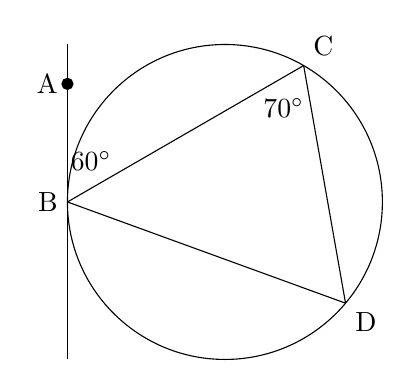
\begin{tikzpicture}
                    \draw (-2,-2) -- (-2,2);
                    \draw (0,0) circle (2cm);
                    \filldraw (-2,1.5) circle (2pt);
                    \coordinate[label=left:A] (A) at (-2, 1.5);
                    \coordinate[label=left:B] (B) at (-2,0);
                    \coordinate[label=above right:C] (C) at (60:2);
                    \coordinate[label=below right:D] (D) at (320:2);
                    \draw (B) -- (C) (C) -- (D) (B) -- (D);
                    \pic["$60^{\circ}$", angle radius=1cm] {angle=C--B--A};
                    \pic["$70^{\circ}$", angle radius=1cm] {angle=B--C--D};
                \end{tikzpicture}
            \end{center}
            \begin{solution}
                We know that $\angle CBD$ is one-half arc $\stackrel{\mbox{\large$\frown$}}{CD}$, but we don't know what arc $\stackrel{\mbox{\large$\frown$}}{CD}$ is.
                We can also find $\angle CBD$ by finding the other two angles of $\triangle CBD$ and subtracting their sum from $180^{\circ}$
                We already have $\angle C$, and $\angle D$ is one-half arc $\stackrel{\mbox{\large$\frown$}}{BC}$.
                Since arc $\stackrel{\mbox{\large$\frown$}}{BC} = 2 \cdot \angle ABC = 120^{\circ}$, we have $\angle D = 60^{\circ}$, and $\angle CBD = 180^{\circ} - \angle C - \angle D = 50^{\circ}$.
            \end{solution}
        \item Segments $PA$ and $PT$ are tangent to the circle.
            Find the measure of $\angle TXA$ if $\angle P = 42^{\circ}$.
            \begin{center}
                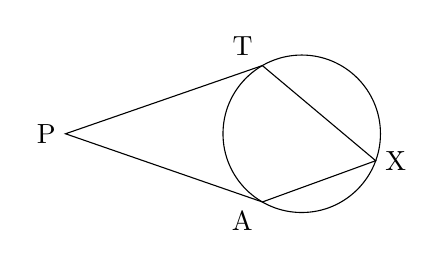
\begin{tikzpicture}
                    \draw (0,0) circle (1cm);
                    \coordinate[label=above left:T] (T) at (120:1);
                    \coordinate[label=left:P] (P) at (180:3);
                    \coordinate[label=below left:A] (A) at (240:1);
                    \coordinate[label=right:X] (X) at (340:1);
                    \draw (T) -- (P) -- (A) -- (X) -- cycle;
                \end{tikzpicture}
            \end{center}
            \begin{solution}
                Let arc $\stackrel{\mbox{\large$\frown$}}{TA} = x$.
                Then arc $\stackrel{\mbox{\large$\frown$}}{TXA} = 360^{\circ} - x$.
                Since $\angle TPA = \frac{\stackrel{\mbox{\large$\frown$}}{TXA} - \stackrel{\mbox{\large$\frown$}}{TA}}{2} = \frac{360 -2x}{2}$, we have $180 - x = 42$, so $x = 138^{\circ}$.
                Since $\angle TXA$ is an inscribed angle, its measure is half that of $\stackrel{\mbox{\large$\frown$}}{TA}$.
                Thus $\angle TXA = 69^{\circ}$.
            \end{solution}
    \end{enumerate}
\end{multicols}
\end{document}